\centering
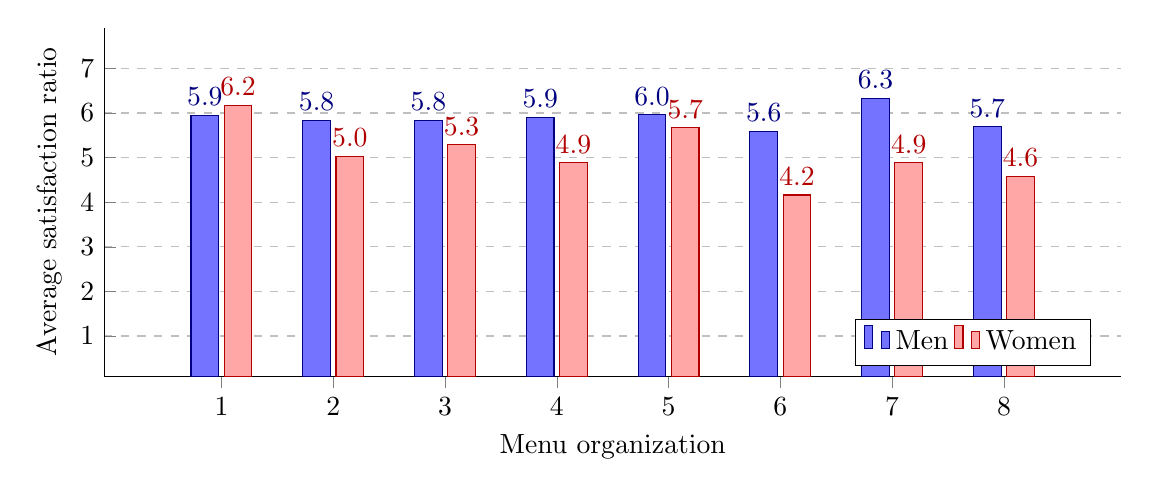
\begin{tikzpicture}
    \begin{axis}[
      %title={Evolution of student participation for each exercise},
      enlarge y limits=false,
      enlarge x limits=-1,
      height=6cm,
      width=14.5cm,
      axis lines*=left,
      xlabel={Menu organization},
      ylabel={Average satisfaction ratio},
      %xmin=1, xmax=4,
      ymin=1, ymax=7,
      xtick=data,
      ytick={1,2,3,4,5,6,7},
      legend pos=south east,
      legend columns=0,
      %xmajorgrids=true,
      ymajorgrids=true,
      grid style=dashed,
      enlargelimits=0.15,
      %histogram related :
      ybar,
      symbolic x coords={1,2,3,4,5,6,7,8},
      nodes near coords,
      every node near coord/.append style={
	  /pgf/number format/fixed zerofill,
	  /pgf/number format/precision=1
      }
      ]
      
    \addplot[blue!50!black, fill=blue!55] coordinates
    {(1,5.9375) (2,5.8333) (3,5.8333) (4,5.8958) (5,5.9583) (6,5.5833) 
     (7,6.3333) (8,5.6875)};
    \addplot[red!70!black, fill=red!35] coordinates
    {(1,6.1666) (2,5.0238) (3,5.2857) (4,4.8809) (5,5.6666) (6,4.16190) 
     (7,4.8809) (8,4.5714)};
    
    \legend{Men, Women}
    
    \end{axis}
  \end{tikzpicture}
  \caption{Average satisfaction ratio for each menu organization according to 
the gender distinction.}